\documentclass[10pt,a4paper]{article}
\usepackage[margin=22mm]{geometry}
\usepackage[T1]{fontenc}
\usepackage{lmodern,amsmath,amssymb,graphicx,booktabs,microtype}
\usepackage[font=small,labelfont=bf]{caption}
\usepackage[hidelinks]{hyperref}
\usepackage{fancyhdr}
\pagestyle{fancy}\fancyhf{}
\fancyhead[L]{\small Computational Mechanics Projects}
\fancyhead[R]{\small FluxLedger}
\fancyfoot[C]{\thepage}
\setlength{\headheight}{14pt}
\setlength{\parindent}{0pt}\setlength{\parskip}{5pt}
\setlength{\emergencystretch}{1em}
\newcommand{\R}{\mathbb{R}}
\title{\vspace{-1.3cm}\LARGE FluxLedger: Auditing Conservation and Numerical Diffusion in Scalar Transport}
\author{\small Computational Mechanics Projects\\\small Reproducible technical research note}
\date{\small 29 September 2026}
\begin{document}\maketitle\thispagestyle{fancy}

\begin{abstract}
Numerical attenuation can resemble physical diffusion even in conservative flow solvers. FluxLedger implements periodic scalar advection--diffusion with a C++17 finite-volume core and Python analysis. First-order upwinding and monotonized-central reconstruction share centered diffusion and strong-stability-preserving Runge--Kutta integration. Exact cell-average Fourier solutions separate discretization error from sampling error; discontinuous pulses test boundedness. Recorded finest-grid orders are 0.978 for upwind advection and 2.001 for limited reconstruction, with maximum smooth-case mass drift $8.31\times10^{-14}$. A Fourier attenuation diagnostic quantifies effective diffusion while explicitly excluding phase accuracy and general material interpretation.
\end{abstract}
\section{Introduction}
A transport scheme should preserve global conservation without creating spurious extrema, yet these properties do not establish accuracy. Upwind transport is robust but dissipative; higher-order reconstruction reduces attenuation while limiting suppresses oscillations near sharp features. This project asks how conservation, boundedness, and diffusion error change under these choices in a controlled one-dimensional setting. The SSP framework~\cite{ssp} provides the time-integration context; the implementation and synthetic experiments are original.
\section{Conservation law and spatial flux}
On a ring of length $L$, constant velocity $a$ and diffusivity $\nu\ge0$ satisfy
\begin{equation}
\partial_tu+\partial_x(au-\nu\partial_xu)=0,\qquad u(x+L,t)=u(x,t).
\end{equation}
The unknowns are cell averages $\bar u_i$ on $N$ uniform cells, not point values. A single shared flux at each face gives
\begin{align}
\dot{\bar u}_i&=-\frac{F_{i+1/2}-F_{i-1/2}}{\Delta x}=R_i(\bar u),\\
F_{i+1/2}&=a u^{\rm up}_{i+1/2}-\nu\frac{\bar u_{i+1}-\bar u_i}{\Delta x}.
\end{align}
Telescoping the flux differences conserves $M=\Delta x\sum_i\bar u_i$ in exact arithmetic. First-order upwind uses piecewise-constant states. The monotonized-central (MC) alternative uses
\begin{equation}
s_i=\operatorname{minmod}\!\left(2\delta_i^-,\frac{\delta_i^-+\delta_i^+}{2},2\delta_i^+\right),
\quad\delta_i^-=\bar u_i-\bar u_{i-1},\quad\delta_i^+=\bar u_{i+1}-\bar u_i.
\end{equation}
Minmod selects the smallest magnitude when signs agree and zero otherwise. Face states are $\bar u_i+s_i/2$ and $\bar u_{i+1}-s_{i+1}/2$; the sign of $a$ selects the upstream value. The standard MC definition is documented independently in Clawpack~\cite{mc}.
\newpage
\section{Time integration and software design}
Reconstruction and fluxes are recomputed at every SSPRK(3,3) stage:
\begin{align}
u^{(1)}&=u^n+\Delta t R(u^n),\\
u^{(2)}&=\tfrac34u^n+\tfrac14[u^{(1)}+\Delta tR(u^{(1)})],\\
u^{n+1}&=\tfrac13u^n+\tfrac23[u^{(2)}+\Delta tR(u^{(2)})].
\end{align}
Both variants use the combined restriction
\begin{equation}
\Delta t_{\max}=\frac{c}{2|a|/\Delta x+2\nu/\Delta x^2},\quad 0<c\le1,
\qquad n_s=\lceil T/\Delta t_{\max}\rceil,\quad\Delta t=T/n_s.
\end{equation}
Thus the input \texttt{cfl} is a fraction of this combined bound. The MC forward-Euler advective coefficient is bounded by $2|a|\Delta t/\Delta x$; adding the two diffusive neighbors gives a convex update under the stated restriction. SSP convex combinations retain boundedness and total-variation properties in this scalar setting, up to roundoff. Zero-duration or zero-transport cases return a copy without steps.

The header-only core computes the numerical solution and its mass ledger. The binding copies input before releasing the Python GIL and returns owned arrays. Scratch storage is allocated once, giving $O(N)$ memory and $O(Nn_s)$ work. Python provides analytical averages, CLI input validation, error analysis, CSV output, and plots. A default step budget rejects excessively expensive requests before integration.
\section{Analytical experiment and observations}
For the initial sine $1+\tfrac12\sin(kx)$, the exact cell average is
\begin{equation}
\bar u_i(t)=1+\tfrac12\operatorname{sinc}(m/N)e^{-\nu k^2t}\sin(k(x_i-at)),
\qquad k=2\pi m/L,
\end{equation}
where $\operatorname{sinc}(z)=\sin(\pi z)/(\pi z)$. Errors use the mean absolute cell-average difference; orders are $\log_2(e_N/e_{2N})$. Twenty-four smooth cases cover advection, diffusion, and their combination; two pulse cases test preservation of $[0,1]$ values.
\begin{center}\begin{tabular}{lrr}\toprule
Finest-grid $L^1$ order & Upwind & MC\\\midrule
Pure advection & 0.97780 & 2.00104\\
Advection--diffusion & 0.98397 & 1.98156\\
Pure diffusion & 1.99997 & 1.99997\\\bottomrule
\end{tabular}\end{center}
Maximum smooth-case mass drift is $8.30\times10^{-14}$, and pulse values stay within $[0,1]$ to the $10^{-12}$ acceptance tolerance. The attenuation diagnostic $\nu_{\rm eff}=-\log|A_1(T)/A_1(0)|/(k^2T)$ uses the fundamental Fourier coefficient. The excess $\nu_{\rm eff}-\nu$ measures damping in that experiment; upwind's leading semidiscrete small-wavenumber excess is $|a|\Delta x/2$.
Figure~\ref{fig:results} visualizes selected recorded diagnostics.
\newpage
\begin{figure}[!ht]\centering
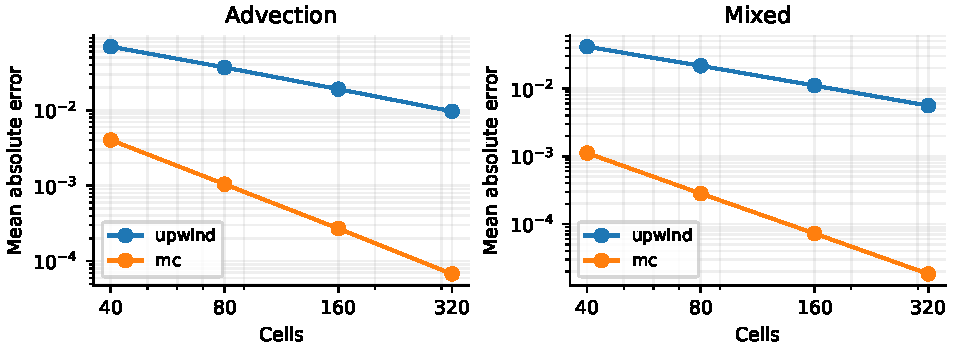
\includegraphics[width=\textwidth]{figure.pdf}
\caption{Recorded cell-average convergence for pure advection and advection--diffusion. MC reconstruction improves the smooth global error rate compared with first-order upwinding.}\label{fig:results}\end{figure}
\section{Discussion and limitations}
The smooth tests recover the expected advantage of MC reconstruction while retaining conservative and bounded pulse transport. Local limiting still reduces accuracy near extrema and discontinuities, so a global second-order $L^1$ rate does not imply pointwise second order. Comparing to point samples instead of cell averages would bias this assessment.

Effective diffusion is a mode-dependent attenuation diagnostic, not a constitutive property or phase-error measure. MC can generate harmonics, and the diagnostic may be negative for some diffusion discretizations. The model has no variable coefficients, boundaries other than periodicity, source terms, nonuniform grids, nonlinear systems, or turbulence. Explicit diffusion requires $O(\Delta x^2)$ steps. Extreme scales and very long integrations are not certified.
\section{Reproducibility and conclusion}
This note documents the committed implementation at \texttt{cd5f603b05b1} and the existing synthetic results; it does not assert new solver runs. Install from the repository root with \texttt{python -m pip install ".[dev]"}; the README gives compiler requirements and verification commands. Code, data, and this manuscript are available at \href{https://github.com/racostacme-come/fluxledger}{the project repository}. No private course material is reproduced. The manuscript was prepared with AI assistance under the project owner\textquotesingle s direction; no peer review is claimed.
Run \texttt{fluxledger campaign --output out}; inspect \texttt{convergence.csv}, profile CSVs, and \texttt{validation.json}. The conclusion is that conservation, boundedness, and attenuation must be reported separately. The shared-flux formulation establishes the mass mechanism, while analytical transport and discontinuous pulses expose different aspects of approximation quality.
\begin{thebibliography}{9}
\bibitem{ssp} S. Gottlieb, C.-W. Shu, and E. Tadmor, Strong stability-preserving high-order time discretization methods, \emph{SIAM Review} 43(1), 89--112 (2001). \href{https://doi.org/10.1137/S003614450036757X}{doi:10.1137/S003614450036757X}.
\bibitem{mc} Clawpack, \emph{TVD limiter functions}, version 5.9 documentation. \href{https://www.clawpack.org/v5.9.x/pyclaw/evolve/limiters.html}{Online documentation}.
\end{thebibliography}

\end{document}
